\documentclass[twoside]{book}

% Packages required by doxygen
\usepackage{fixltx2e}
\usepackage{calc}
\usepackage{doxygen}
\usepackage[export]{adjustbox} % also loads graphicx
\usepackage{graphicx}
\usepackage[utf8]{inputenc}
\usepackage{makeidx}
\usepackage{multicol}
\usepackage{multirow}
\PassOptionsToPackage{warn}{textcomp}
\usepackage{textcomp}
\usepackage[nointegrals]{wasysym}
\usepackage[table]{xcolor}

% Font selection
\usepackage[T1]{fontenc}
\usepackage[scaled=.90]{helvet}
\usepackage{courier}
\usepackage{amssymb}
\usepackage{sectsty}
\renewcommand{\familydefault}{\sfdefault}
\allsectionsfont{%
  \fontseries{bc}\selectfont%
  \color{darkgray}%
}
\renewcommand{\DoxyLabelFont}{%
  \fontseries{bc}\selectfont%
  \color{darkgray}%
}
\newcommand{\+}{\discretionary{\mbox{\scriptsize$\hookleftarrow$}}{}{}}

% Page & text layout
\usepackage{geometry}
\geometry{%
  a4paper,%
  top=2.5cm,%
  bottom=2.5cm,%
  left=2.5cm,%
  right=2.5cm%
}
\tolerance=750
\hfuzz=15pt
\hbadness=750
\setlength{\emergencystretch}{15pt}
\setlength{\parindent}{0cm}
\setlength{\parskip}{3ex plus 2ex minus 2ex}
\makeatletter
\renewcommand{\paragraph}{%
  \@startsection{paragraph}{4}{0ex}{-1.0ex}{1.0ex}{%
    \normalfont\normalsize\bfseries\SS@parafont%
  }%
}
\renewcommand{\subparagraph}{%
  \@startsection{subparagraph}{5}{0ex}{-1.0ex}{1.0ex}{%
    \normalfont\normalsize\bfseries\SS@subparafont%
  }%
}
\makeatother

% Headers & footers
\usepackage{fancyhdr}
\pagestyle{fancyplain}
\fancyhead[LE]{\fancyplain{}{\bfseries\thepage}}
\fancyhead[CE]{\fancyplain{}{}}
\fancyhead[RE]{\fancyplain{}{\bfseries\leftmark}}
\fancyhead[LO]{\fancyplain{}{\bfseries\rightmark}}
\fancyhead[CO]{\fancyplain{}{}}
\fancyhead[RO]{\fancyplain{}{\bfseries\thepage}}
\fancyfoot[LE]{\fancyplain{}{}}
\fancyfoot[CE]{\fancyplain{}{}}
\fancyfoot[RE]{\fancyplain{}{\bfseries\scriptsize Generated by Doxygen }}
\fancyfoot[LO]{\fancyplain{}{\bfseries\scriptsize Generated by Doxygen }}
\fancyfoot[CO]{\fancyplain{}{}}
\fancyfoot[RO]{\fancyplain{}{}}
\renewcommand{\footrulewidth}{0.4pt}
\renewcommand{\chaptermark}[1]{%
  \markboth{#1}{}%
}
\renewcommand{\sectionmark}[1]{%
  \markright{\thesection\ #1}%
}

% Indices & bibliography
\usepackage{natbib}
\usepackage[titles]{tocloft}
\setcounter{tocdepth}{3}
\setcounter{secnumdepth}{5}
\makeindex

% Hyperlinks (required, but should be loaded last)
\usepackage{ifpdf}
\ifpdf
  \usepackage[pdftex,pagebackref=true]{hyperref}
\else
  \usepackage[ps2pdf,pagebackref=true]{hyperref}
\fi
\hypersetup{%
  colorlinks=true,%
  linkcolor=blue,%
  citecolor=blue,%
  unicode%
}

% Custom commands
\newcommand{\clearemptydoublepage}{%
  \newpage{\pagestyle{empty}\cleardoublepage}%
}

\usepackage{caption}
\captionsetup{labelsep=space,justification=centering,font={bf},singlelinecheck=off,skip=4pt,position=top}

%===== C O N T E N T S =====

\begin{document}

% Titlepage & ToC
\hypersetup{pageanchor=false,
             bookmarksnumbered=true,
             pdfencoding=unicode
            }
\pagenumbering{roman}
\begin{titlepage}
\vspace*{7cm}
\begin{center}%
{\Large My Project }\\
\vspace*{1cm}
{\large Generated by Doxygen 1.8.11}\\
\end{center}
\end{titlepage}
\clearemptydoublepage
\tableofcontents
\clearemptydoublepage
\pagenumbering{arabic}
\hypersetup{pageanchor=true}

%--- Begin generated contents ---
\chapter{Namespace Index}
\section{Namespace List}
Here is a list of all namespaces with brief descriptions\+:\begin{DoxyCompactList}
\item\contentsline{section}{\hyperlink{namespacequeuesavitch}{queuesavitch} }{\pageref{namespacequeuesavitch}}{}
\end{DoxyCompactList}

\chapter{Hierarchical Index}
\section{Class Hierarchy}
This inheritance list is sorted roughly, but not completely, alphabetically\+:\begin{DoxyCompactList}
\item \contentsline{section}{Fruit}{\pageref{classFruit}}{}
\begin{DoxyCompactList}
\item \contentsline{section}{Apple}{\pageref{classApple}}{}
\item \contentsline{section}{Grape}{\pageref{classGrape}}{}
\item \contentsline{section}{Orange}{\pageref{classOrange}}{}
\end{DoxyCompactList}
\item \contentsline{section}{List}{\pageref{classList}}{}
\item \contentsline{section}{List\+:\+:Node}{\pageref{structList_1_1Node}}{}
\end{DoxyCompactList}

\chapter{Class Index}
\section{Class List}
Here are the classes, structs, unions and interfaces with brief descriptions\+:\begin{DoxyCompactList}
\item\contentsline{section}{\hyperlink{structnode}{node} }{\pageref{structnode}}{}
\item\contentsline{section}{\hyperlink{structnode1}{node1} }{\pageref{structnode1}}{}
\item\contentsline{section}{\hyperlink{structnode__info}{node\+\_\+info} }{\pageref{structnode__info}}{}
\end{DoxyCompactList}

\chapter{File Index}
\section{File List}
Here is a list of all files with brief descriptions\+:\begin{DoxyCompactList}
\item\contentsline{section}{\hyperlink{Lab1_8c}{Lab1.\+c} }{\pageref{Lab1_8c}}{}
\end{DoxyCompactList}

\chapter{Namespace Documentation}
\hypertarget{namespacewikibooks__design__patterns}{}\section{wikibooks\+\_\+design\+\_\+patterns Namespace Reference}
\label{namespacewikibooks__design__patterns}\index{wikibooks\+\_\+design\+\_\+patterns@{wikibooks\+\_\+design\+\_\+patterns}}
\subsection*{Classes}
\begin{DoxyCompactItemize}
\item 
class \hyperlink{classwikibooks__design__patterns_1_1Evaluator}{Evaluator}
\item 
struct \hyperlink{structwikibooks__design__patterns_1_1Expression}{Expression}
\item 
class \hyperlink{classwikibooks__design__patterns_1_1Minus}{Minus}
\item 
class \hyperlink{classwikibooks__design__patterns_1_1Number}{Number}
\item 
class \hyperlink{classwikibooks__design__patterns_1_1Plus}{Plus}
\item 
class \hyperlink{classwikibooks__design__patterns_1_1Variable}{Variable}
\end{DoxyCompactItemize}
\subsection*{Typedefs}
\begin{DoxyCompactItemize}
\item 
typedef std\+::string \hyperlink{namespacewikibooks__design__patterns_a603d2591ea56686888d0e4389481a453}{String}
\item 
typedef std\+::map$<$ \hyperlink{namespacewikibooks__design__patterns_a603d2591ea56686888d0e4389481a453}{String}, \hyperlink{structwikibooks__design__patterns_1_1Expression}{Expression} $\ast$ $>$ \hyperlink{namespacewikibooks__design__patterns_adf1889a865861dea765d8a115cc66ae9}{Map}
\item 
typedef std\+::list$<$ \hyperlink{structwikibooks__design__patterns_1_1Expression}{Expression} $\ast$ $>$ \hyperlink{namespacewikibooks__design__patterns_a3247979de240b19de03793d4ec6ede0e}{Stack}
\end{DoxyCompactItemize}


\subsection{Typedef Documentation}
\index{wikibooks\+\_\+design\+\_\+patterns@{wikibooks\+\_\+design\+\_\+patterns}!Map@{Map}}
\index{Map@{Map}!wikibooks\+\_\+design\+\_\+patterns@{wikibooks\+\_\+design\+\_\+patterns}}
\subsubsection[{\texorpdfstring{Map}{Map}}]{\setlength{\rightskip}{0pt plus 5cm}typedef std\+::map$<${\bf String},{\bf Expression}$\ast$$>$ {\bf wikibooks\+\_\+design\+\_\+patterns\+::\+Map}}\hypertarget{namespacewikibooks__design__patterns_adf1889a865861dea765d8a115cc66ae9}{}\label{namespacewikibooks__design__patterns_adf1889a865861dea765d8a115cc66ae9}
\index{wikibooks\+\_\+design\+\_\+patterns@{wikibooks\+\_\+design\+\_\+patterns}!Stack@{Stack}}
\index{Stack@{Stack}!wikibooks\+\_\+design\+\_\+patterns@{wikibooks\+\_\+design\+\_\+patterns}}
\subsubsection[{\texorpdfstring{Stack}{Stack}}]{\setlength{\rightskip}{0pt plus 5cm}typedef std\+::list$<${\bf Expression}$\ast$$>$ {\bf wikibooks\+\_\+design\+\_\+patterns\+::\+Stack}}\hypertarget{namespacewikibooks__design__patterns_a3247979de240b19de03793d4ec6ede0e}{}\label{namespacewikibooks__design__patterns_a3247979de240b19de03793d4ec6ede0e}
\index{wikibooks\+\_\+design\+\_\+patterns@{wikibooks\+\_\+design\+\_\+patterns}!String@{String}}
\index{String@{String}!wikibooks\+\_\+design\+\_\+patterns@{wikibooks\+\_\+design\+\_\+patterns}}
\subsubsection[{\texorpdfstring{String}{String}}]{\setlength{\rightskip}{0pt plus 5cm}typedef std\+::string {\bf wikibooks\+\_\+design\+\_\+patterns\+::\+String}}\hypertarget{namespacewikibooks__design__patterns_a603d2591ea56686888d0e4389481a453}{}\label{namespacewikibooks__design__patterns_a603d2591ea56686888d0e4389481a453}

\chapter{Class Documentation}
\hypertarget{classwikibooks__design__patterns_1_1Chess}{}\section{wikibooks\+\_\+design\+\_\+patterns\+:\+:Chess Class Reference}
\label{classwikibooks__design__patterns_1_1Chess}\index{wikibooks\+\_\+design\+\_\+patterns\+::\+Chess@{wikibooks\+\_\+design\+\_\+patterns\+::\+Chess}}


Inheritance diagram for wikibooks\+\_\+design\+\_\+patterns\+:\+:Chess\+:
\nopagebreak
\begin{figure}[H]
\begin{center}
\leavevmode
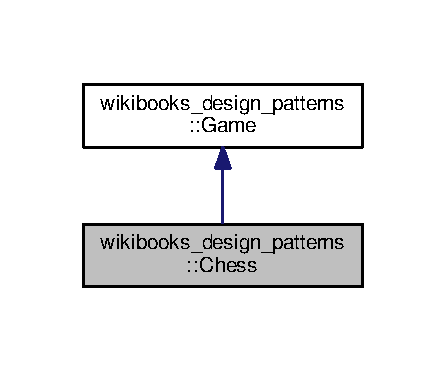
\includegraphics[width=214pt]{classwikibooks__design__patterns_1_1Chess__inherit__graph}
\end{center}
\end{figure}


Collaboration diagram for wikibooks\+\_\+design\+\_\+patterns\+:\+:Chess\+:
\nopagebreak
\begin{figure}[H]
\begin{center}
\leavevmode
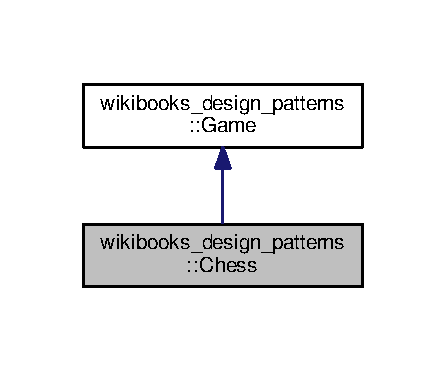
\includegraphics[width=214pt]{classwikibooks__design__patterns_1_1Chess__coll__graph}
\end{center}
\end{figure}
\subsection*{Private Types}
\begin{DoxyCompactItemize}
\item 
enum \{ \hyperlink{classwikibooks__design__patterns_1_1Chess_a4dd06f0e46a019fabaa0d06013eda2ecaf2a5dc2ad13559326bb03ee0772d95c0}{M\+O\+V\+E\+S\+\_\+\+W\+I\+N\+\_\+\+C\+O\+R\+R\+E\+C\+T\+I\+ON} = 7
 \}
\end{DoxyCompactItemize}
\subsection*{Private Member Functions}
\begin{DoxyCompactItemize}
\item 
void \hyperlink{classwikibooks__design__patterns_1_1Chess_ab90b8fa2a95ad530b286d0c991ee85b7}{initialize\+Game} ()
\item 
void \hyperlink{classwikibooks__design__patterns_1_1Chess_ac0c6d94fab2c7f8ca8995591a3b688ed}{make\+Play} (int player)
\item 
bool \hyperlink{classwikibooks__design__patterns_1_1Chess_a7722fa3719cef20836f15b9579dfb8db}{end\+Of\+Game} ()
\item 
void \hyperlink{classwikibooks__design__patterns_1_1Chess_a0a38a15831a76736781e8952eeca43d4}{print\+Winner} ()
\end{DoxyCompactItemize}
\subsection*{Additional Inherited Members}


\subsection{Member Enumeration Documentation}
\subsubsection[{\texorpdfstring{anonymous enum}{anonymous enum}}]{\setlength{\rightskip}{0pt plus 5cm}anonymous enum\hspace{0.3cm}{\ttfamily [private]}}\hypertarget{classwikibooks__design__patterns_1_1Chess_a4dd06f0e46a019fabaa0d06013eda2ec}{}\label{classwikibooks__design__patterns_1_1Chess_a4dd06f0e46a019fabaa0d06013eda2ec}
\begin{Desc}
\item[Enumerator]\par
\begin{description}
\index{M\+O\+V\+E\+S\+\_\+\+W\+I\+N\+\_\+\+C\+O\+R\+R\+E\+C\+T\+I\+ON@{M\+O\+V\+E\+S\+\_\+\+W\+I\+N\+\_\+\+C\+O\+R\+R\+E\+C\+T\+I\+ON}!wikibooks\+\_\+design\+\_\+patterns\+::\+Chess@{wikibooks\+\_\+design\+\_\+patterns\+::\+Chess}}\index{wikibooks\+\_\+design\+\_\+patterns\+::\+Chess@{wikibooks\+\_\+design\+\_\+patterns\+::\+Chess}!M\+O\+V\+E\+S\+\_\+\+W\+I\+N\+\_\+\+C\+O\+R\+R\+E\+C\+T\+I\+ON@{M\+O\+V\+E\+S\+\_\+\+W\+I\+N\+\_\+\+C\+O\+R\+R\+E\+C\+T\+I\+ON}}\item[{\em 
M\+O\+V\+E\+S\+\_\+\+W\+I\+N\+\_\+\+C\+O\+R\+R\+E\+C\+T\+I\+ON\hypertarget{classwikibooks__design__patterns_1_1Chess_a4dd06f0e46a019fabaa0d06013eda2ecaf2a5dc2ad13559326bb03ee0772d95c0}{}\label{classwikibooks__design__patterns_1_1Chess_a4dd06f0e46a019fabaa0d06013eda2ecaf2a5dc2ad13559326bb03ee0772d95c0}
}]\end{description}
\end{Desc}

\begin{DoxyCode}
145     \{
146     \hyperlink{classwikibooks__design__patterns_1_1Chess_a4dd06f0e46a019fabaa0d06013eda2ecaf2a5dc2ad13559326bb03ee0772d95c0}{MOVES\_WIN\_CORRECTION} = 7,
147     \};
\end{DoxyCode}


\subsection{Member Function Documentation}
\index{wikibooks\+\_\+design\+\_\+patterns\+::\+Chess@{wikibooks\+\_\+design\+\_\+patterns\+::\+Chess}!end\+Of\+Game@{end\+Of\+Game}}
\index{end\+Of\+Game@{end\+Of\+Game}!wikibooks\+\_\+design\+\_\+patterns\+::\+Chess@{wikibooks\+\_\+design\+\_\+patterns\+::\+Chess}}
\subsubsection[{\texorpdfstring{end\+Of\+Game()}{endOfGame()}}]{\setlength{\rightskip}{0pt plus 5cm}bool wikibooks\+\_\+design\+\_\+patterns\+::\+Chess\+::end\+Of\+Game (
\begin{DoxyParamCaption}
{}
\end{DoxyParamCaption}
)\hspace{0.3cm}{\ttfamily [inline]}, {\ttfamily [private]}, {\ttfamily [virtual]}}\hypertarget{classwikibooks__design__patterns_1_1Chess_a7722fa3719cef20836f15b9579dfb8db}{}\label{classwikibooks__design__patterns_1_1Chess_a7722fa3719cef20836f15b9579dfb8db}


Implements \hyperlink{classwikibooks__design__patterns_1_1Game_a351f5fb200c6b26d5b6150f1f09bc87d}{wikibooks\+\_\+design\+\_\+patterns\+::\+Game}.


\begin{DoxyCode}
130                      \{
131         \textcolor{comment}{// Return true if in Checkmate or }
132         \textcolor{comment}{// Stalemate has been reached}
133     \textcolor{keywordflow}{return} (-1 != \hyperlink{classwikibooks__design__patterns_1_1Game_a6385d85f068769843e22f7741a4ae154}{playerWon});
134     \}
\end{DoxyCode}
\index{wikibooks\+\_\+design\+\_\+patterns\+::\+Chess@{wikibooks\+\_\+design\+\_\+patterns\+::\+Chess}!initialize\+Game@{initialize\+Game}}
\index{initialize\+Game@{initialize\+Game}!wikibooks\+\_\+design\+\_\+patterns\+::\+Chess@{wikibooks\+\_\+design\+\_\+patterns\+::\+Chess}}
\subsubsection[{\texorpdfstring{initialize\+Game()}{initializeGame()}}]{\setlength{\rightskip}{0pt plus 5cm}void wikibooks\+\_\+design\+\_\+patterns\+::\+Chess\+::initialize\+Game (
\begin{DoxyParamCaption}
{}
\end{DoxyParamCaption}
)\hspace{0.3cm}{\ttfamily [inline]}, {\ttfamily [private]}, {\ttfamily [virtual]}}\hypertarget{classwikibooks__design__patterns_1_1Chess_ab90b8fa2a95ad530b286d0c991ee85b7}{}\label{classwikibooks__design__patterns_1_1Chess_ab90b8fa2a95ad530b286d0c991ee85b7}


Implements \hyperlink{classwikibooks__design__patterns_1_1Game_a77c50ee852af77bb15d46ba0a39683c4}{wikibooks\+\_\+design\+\_\+patterns\+::\+Game}.


\begin{DoxyCode}
111                           \{
112         \textcolor{comment}{// Initialize players}
113     \hyperlink{classwikibooks__design__patterns_1_1Game_a8641adb02e0f068ff9ecb6c375562d7b}{playersCount} = 2;
114         \textcolor{comment}{// Put the pieces on the board}
115     \}
\end{DoxyCode}
\index{wikibooks\+\_\+design\+\_\+patterns\+::\+Chess@{wikibooks\+\_\+design\+\_\+patterns\+::\+Chess}!make\+Play@{make\+Play}}
\index{make\+Play@{make\+Play}!wikibooks\+\_\+design\+\_\+patterns\+::\+Chess@{wikibooks\+\_\+design\+\_\+patterns\+::\+Chess}}
\subsubsection[{\texorpdfstring{make\+Play(int player)}{makePlay(int player)}}]{\setlength{\rightskip}{0pt plus 5cm}void wikibooks\+\_\+design\+\_\+patterns\+::\+Chess\+::make\+Play (
\begin{DoxyParamCaption}
\item[{int}]{player}
\end{DoxyParamCaption}
)\hspace{0.3cm}{\ttfamily [inline]}, {\ttfamily [private]}, {\ttfamily [virtual]}}\hypertarget{classwikibooks__design__patterns_1_1Chess_ac0c6d94fab2c7f8ca8995591a3b688ed}{}\label{classwikibooks__design__patterns_1_1Chess_ac0c6d94fab2c7f8ca8995591a3b688ed}


Implements \hyperlink{classwikibooks__design__patterns_1_1Game_ab1859f681536780d02da57634e963d4a}{wikibooks\+\_\+design\+\_\+patterns\+::\+Game}.


\begin{DoxyCode}
116                               \{
117     assert(player < \hyperlink{classwikibooks__design__patterns_1_1Game_a8641adb02e0f068ff9ecb6c375562d7b}{playersCount});
118 
119         \textcolor{comment}{// Process a turn for the player}
120 
121     \textcolor{comment}{//  decide winner}
122     \textcolor{keywordflow}{if} (\hyperlink{classwikibooks__design__patterns_1_1Game_ac7bac015fe2e5ead905f7fb8ae63d3aa}{movesCount} < 2)
123         \textcolor{keywordflow}{return};
124     \textcolor{keyword}{const} \textcolor{keywordtype}{int} chances = (\hyperlink{classwikibooks__design__patterns_1_1Game_ac7bac015fe2e5ead905f7fb8ae63d3aa}{movesCount} > 99) ? 99 : \hyperlink{classwikibooks__design__patterns_1_1Game_ac7bac015fe2e5ead905f7fb8ae63d3aa}{movesCount};
125     \textcolor{keyword}{const} \textcolor{keywordtype}{int} random = \hyperlink{classwikibooks__design__patterns_1_1Chess_a4dd06f0e46a019fabaa0d06013eda2ecaf2a5dc2ad13559326bb03ee0772d95c0}{MOVES\_WIN\_CORRECTION} * rand() * 100 / RAND\_MAX;
126     \textcolor{comment}{//std::cout<<random<<" : "<<chances<<std::endl;}
127     \textcolor{keywordflow}{if} (random < chances)
128         \hyperlink{classwikibooks__design__patterns_1_1Game_a6385d85f068769843e22f7741a4ae154}{playerWon} = player;
129     \}
\end{DoxyCode}
\index{wikibooks\+\_\+design\+\_\+patterns\+::\+Chess@{wikibooks\+\_\+design\+\_\+patterns\+::\+Chess}!print\+Winner@{print\+Winner}}
\index{print\+Winner@{print\+Winner}!wikibooks\+\_\+design\+\_\+patterns\+::\+Chess@{wikibooks\+\_\+design\+\_\+patterns\+::\+Chess}}
\subsubsection[{\texorpdfstring{print\+Winner()}{printWinner()}}]{\setlength{\rightskip}{0pt plus 5cm}void wikibooks\+\_\+design\+\_\+patterns\+::\+Chess\+::print\+Winner (
\begin{DoxyParamCaption}
{}
\end{DoxyParamCaption}
)\hspace{0.3cm}{\ttfamily [inline]}, {\ttfamily [private]}, {\ttfamily [virtual]}}\hypertarget{classwikibooks__design__patterns_1_1Chess_a0a38a15831a76736781e8952eeca43d4}{}\label{classwikibooks__design__patterns_1_1Chess_a0a38a15831a76736781e8952eeca43d4}


Implements \hyperlink{classwikibooks__design__patterns_1_1Game_a98d860c143cb793b4c1cb630d9314cba}{wikibooks\+\_\+design\+\_\+patterns\+::\+Game}.


\begin{DoxyCode}
135                        \{
136     assert(\hyperlink{classwikibooks__design__patterns_1_1Game_a6385d85f068769843e22f7741a4ae154}{playerWon} >= 0);
137     assert(\hyperlink{classwikibooks__design__patterns_1_1Game_a6385d85f068769843e22f7741a4ae154}{playerWon} < \hyperlink{classwikibooks__design__patterns_1_1Game_a8641adb02e0f068ff9ecb6c375562d7b}{playersCount});
138 
139         \textcolor{comment}{// Display the winning player}
140     std::cout<<\textcolor{stringliteral}{"Player "}<<\hyperlink{classwikibooks__design__patterns_1_1Game_a6385d85f068769843e22f7741a4ae154}{playerWon}<<\textcolor{stringliteral}{" won in "}<<\hyperlink{classwikibooks__design__patterns_1_1Game_ac7bac015fe2e5ead905f7fb8ae63d3aa}{movesCount}<<\textcolor{stringliteral}{" moves."}<<std::endl;
141     \}
\end{DoxyCode}


The documentation for this class was generated from the following file\+:\begin{DoxyCompactItemize}
\item 
\hyperlink{Template_8cpp}{Template.\+cpp}\end{DoxyCompactItemize}

\hypertarget{classwikibooks__design__patterns_1_1Game}{}\section{wikibooks\+\_\+design\+\_\+patterns\+:\+:Game Class Reference}
\label{classwikibooks__design__patterns_1_1Game}\index{wikibooks\+\_\+design\+\_\+patterns\+::\+Game@{wikibooks\+\_\+design\+\_\+patterns\+::\+Game}}


Inheritance diagram for wikibooks\+\_\+design\+\_\+patterns\+:\+:Game\+:
\nopagebreak
\begin{figure}[H]
\begin{center}
\leavevmode
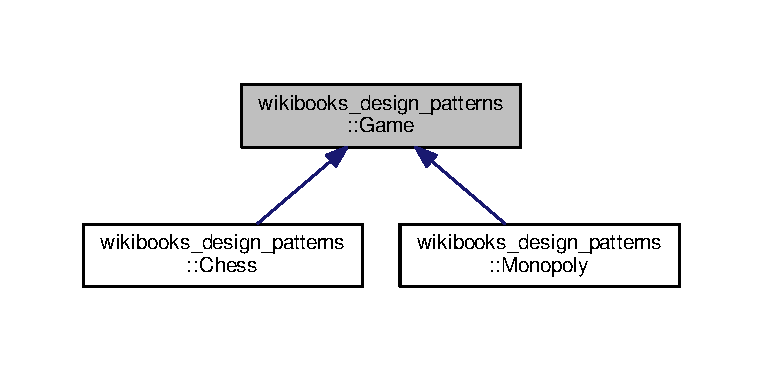
\includegraphics[width=350pt]{classwikibooks__design__patterns_1_1Game__inherit__graph}
\end{center}
\end{figure}
\subsection*{Public Member Functions}
\begin{DoxyCompactItemize}
\item 
\hyperlink{classwikibooks__design__patterns_1_1Game_acdfcc4d37f30a39ed438b81de8e00046}{Game} ()
\item 
void \hyperlink{classwikibooks__design__patterns_1_1Game_adaf21d3c4d07388f1cba12092ced5d38}{play\+One\+Game} (const int \hyperlink{classwikibooks__design__patterns_1_1Game_a8641adb02e0f068ff9ecb6c375562d7b}{players\+Count}=0)
\end{DoxyCompactItemize}
\subsection*{Protected Member Functions}
\begin{DoxyCompactItemize}
\item 
virtual void \hyperlink{classwikibooks__design__patterns_1_1Game_a77c50ee852af77bb15d46ba0a39683c4}{initialize\+Game} ()=0
\item 
virtual void \hyperlink{classwikibooks__design__patterns_1_1Game_ab1859f681536780d02da57634e963d4a}{make\+Play} (int player)=0
\item 
virtual bool \hyperlink{classwikibooks__design__patterns_1_1Game_a351f5fb200c6b26d5b6150f1f09bc87d}{end\+Of\+Game} ()=0
\item 
virtual void \hyperlink{classwikibooks__design__patterns_1_1Game_a98d860c143cb793b4c1cb630d9314cba}{print\+Winner} ()=0
\end{DoxyCompactItemize}
\subsection*{Protected Attributes}
\begin{DoxyCompactItemize}
\item 
int \hyperlink{classwikibooks__design__patterns_1_1Game_a8641adb02e0f068ff9ecb6c375562d7b}{players\+Count}
\item 
int \hyperlink{classwikibooks__design__patterns_1_1Game_ac7bac015fe2e5ead905f7fb8ae63d3aa}{moves\+Count}
\item 
int \hyperlink{classwikibooks__design__patterns_1_1Game_a6385d85f068769843e22f7741a4ae154}{player\+Won}
\end{DoxyCompactItemize}
\subsection*{Private Member Functions}
\begin{DoxyCompactItemize}
\item 
void \hyperlink{classwikibooks__design__patterns_1_1Game_a3de3408a468266ea25ba26b8e27544e3}{Initialize\+Game} ()
\end{DoxyCompactItemize}


\subsection{Detailed Description}
An abstract class that is common to several games in which players play against the others, but only one is playing at a given time. 

\subsection{Constructor \& Destructor Documentation}
\index{wikibooks\+\_\+design\+\_\+patterns\+::\+Game@{wikibooks\+\_\+design\+\_\+patterns\+::\+Game}!Game@{Game}}
\index{Game@{Game}!wikibooks\+\_\+design\+\_\+patterns\+::\+Game@{wikibooks\+\_\+design\+\_\+patterns\+::\+Game}}
\subsubsection[{\texorpdfstring{Game()}{Game()}}]{\setlength{\rightskip}{0pt plus 5cm}wikibooks\+\_\+design\+\_\+patterns\+::\+Game\+::\+Game (
\begin{DoxyParamCaption}
{}
\end{DoxyParamCaption}
)\hspace{0.3cm}{\ttfamily [inline]}}\hypertarget{classwikibooks__design__patterns_1_1Game_acdfcc4d37f30a39ed438b81de8e00046}{}\label{classwikibooks__design__patterns_1_1Game_acdfcc4d37f30a39ed438b81de8e00046}

\begin{DoxyCode}
16           : \hyperlink{classwikibooks__design__patterns_1_1Game_a8641adb02e0f068ff9ecb6c375562d7b}{playersCount}(0), \hyperlink{classwikibooks__design__patterns_1_1Game_ac7bac015fe2e5ead905f7fb8ae63d3aa}{movesCount}(0), \hyperlink{classwikibooks__design__patterns_1_1Game_a6385d85f068769843e22f7741a4ae154}{playerWon}(-1)
17     \{
18         srand( (\textcolor{keywordtype}{unsigned})time( NULL));
19     \}
\end{DoxyCode}


\subsection{Member Function Documentation}
\index{wikibooks\+\_\+design\+\_\+patterns\+::\+Game@{wikibooks\+\_\+design\+\_\+patterns\+::\+Game}!end\+Of\+Game@{end\+Of\+Game}}
\index{end\+Of\+Game@{end\+Of\+Game}!wikibooks\+\_\+design\+\_\+patterns\+::\+Game@{wikibooks\+\_\+design\+\_\+patterns\+::\+Game}}
\subsubsection[{\texorpdfstring{end\+Of\+Game()=0}{endOfGame()=0}}]{\setlength{\rightskip}{0pt plus 5cm}virtual bool wikibooks\+\_\+design\+\_\+patterns\+::\+Game\+::end\+Of\+Game (
\begin{DoxyParamCaption}
{}
\end{DoxyParamCaption}
)\hspace{0.3cm}{\ttfamily [protected]}, {\ttfamily [pure virtual]}}\hypertarget{classwikibooks__design__patterns_1_1Game_a351f5fb200c6b26d5b6150f1f09bc87d}{}\label{classwikibooks__design__patterns_1_1Game_a351f5fb200c6b26d5b6150f1f09bc87d}


Implemented in \hyperlink{classwikibooks__design__patterns_1_1Chess_a7722fa3719cef20836f15b9579dfb8db}{wikibooks\+\_\+design\+\_\+patterns\+::\+Chess}, and \hyperlink{classwikibooks__design__patterns_1_1Monopoly_ab533fb92f64065d8cae9a731e6fe789d}{wikibooks\+\_\+design\+\_\+patterns\+::\+Monopoly}.

\index{wikibooks\+\_\+design\+\_\+patterns\+::\+Game@{wikibooks\+\_\+design\+\_\+patterns\+::\+Game}!initialize\+Game@{initialize\+Game}}
\index{initialize\+Game@{initialize\+Game}!wikibooks\+\_\+design\+\_\+patterns\+::\+Game@{wikibooks\+\_\+design\+\_\+patterns\+::\+Game}}
\subsubsection[{\texorpdfstring{initialize\+Game()=0}{initializeGame()=0}}]{\setlength{\rightskip}{0pt plus 5cm}virtual void wikibooks\+\_\+design\+\_\+patterns\+::\+Game\+::initialize\+Game (
\begin{DoxyParamCaption}
{}
\end{DoxyParamCaption}
)\hspace{0.3cm}{\ttfamily [protected]}, {\ttfamily [pure virtual]}}\hypertarget{classwikibooks__design__patterns_1_1Game_a77c50ee852af77bb15d46ba0a39683c4}{}\label{classwikibooks__design__patterns_1_1Game_a77c50ee852af77bb15d46ba0a39683c4}


Implemented in \hyperlink{classwikibooks__design__patterns_1_1Chess_ab90b8fa2a95ad530b286d0c991ee85b7}{wikibooks\+\_\+design\+\_\+patterns\+::\+Chess}, and \hyperlink{classwikibooks__design__patterns_1_1Monopoly_a9fa4e1a5c85d7b9f1e2b1fdf4d1911ab}{wikibooks\+\_\+design\+\_\+patterns\+::\+Monopoly}.

\index{wikibooks\+\_\+design\+\_\+patterns\+::\+Game@{wikibooks\+\_\+design\+\_\+patterns\+::\+Game}!Initialize\+Game@{Initialize\+Game}}
\index{Initialize\+Game@{Initialize\+Game}!wikibooks\+\_\+design\+\_\+patterns\+::\+Game@{wikibooks\+\_\+design\+\_\+patterns\+::\+Game}}
\subsubsection[{\texorpdfstring{Initialize\+Game()}{InitializeGame()}}]{\setlength{\rightskip}{0pt plus 5cm}void wikibooks\+\_\+design\+\_\+patterns\+::\+Game\+::\+Initialize\+Game (
\begin{DoxyParamCaption}
{}
\end{DoxyParamCaption}
)\hspace{0.3cm}{\ttfamily [inline]}, {\ttfamily [private]}}\hypertarget{classwikibooks__design__patterns_1_1Game_a3de3408a468266ea25ba26b8e27544e3}{}\label{classwikibooks__design__patterns_1_1Game_a3de3408a468266ea25ba26b8e27544e3}

\begin{DoxyCode}
53     \{
54         \hyperlink{classwikibooks__design__patterns_1_1Game_ac7bac015fe2e5ead905f7fb8ae63d3aa}{movesCount} = 0;
55         \hyperlink{classwikibooks__design__patterns_1_1Game_a6385d85f068769843e22f7741a4ae154}{playerWon} = -1;
56 
57         \hyperlink{classwikibooks__design__patterns_1_1Game_a77c50ee852af77bb15d46ba0a39683c4}{initializeGame}();
58     \}
\end{DoxyCode}


Here is the call graph for this function\+:
\nopagebreak
\begin{figure}[H]
\begin{center}
\leavevmode
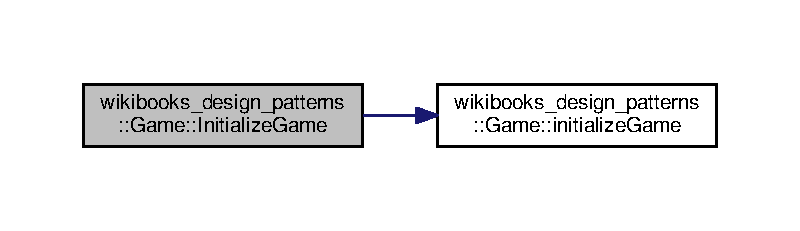
\includegraphics[width=350pt]{classwikibooks__design__patterns_1_1Game_a3de3408a468266ea25ba26b8e27544e3_cgraph}
\end{center}
\end{figure}


\index{wikibooks\+\_\+design\+\_\+patterns\+::\+Game@{wikibooks\+\_\+design\+\_\+patterns\+::\+Game}!make\+Play@{make\+Play}}
\index{make\+Play@{make\+Play}!wikibooks\+\_\+design\+\_\+patterns\+::\+Game@{wikibooks\+\_\+design\+\_\+patterns\+::\+Game}}
\subsubsection[{\texorpdfstring{make\+Play(int player)=0}{makePlay(int player)=0}}]{\setlength{\rightskip}{0pt plus 5cm}virtual void wikibooks\+\_\+design\+\_\+patterns\+::\+Game\+::make\+Play (
\begin{DoxyParamCaption}
\item[{int}]{player}
\end{DoxyParamCaption}
)\hspace{0.3cm}{\ttfamily [protected]}, {\ttfamily [pure virtual]}}\hypertarget{classwikibooks__design__patterns_1_1Game_ab1859f681536780d02da57634e963d4a}{}\label{classwikibooks__design__patterns_1_1Game_ab1859f681536780d02da57634e963d4a}


Implemented in \hyperlink{classwikibooks__design__patterns_1_1Chess_ac0c6d94fab2c7f8ca8995591a3b688ed}{wikibooks\+\_\+design\+\_\+patterns\+::\+Chess}, and \hyperlink{classwikibooks__design__patterns_1_1Monopoly_ab885dd62ab49fba54bd2ce542702caaa}{wikibooks\+\_\+design\+\_\+patterns\+::\+Monopoly}.

\index{wikibooks\+\_\+design\+\_\+patterns\+::\+Game@{wikibooks\+\_\+design\+\_\+patterns\+::\+Game}!play\+One\+Game@{play\+One\+Game}}
\index{play\+One\+Game@{play\+One\+Game}!wikibooks\+\_\+design\+\_\+patterns\+::\+Game@{wikibooks\+\_\+design\+\_\+patterns\+::\+Game}}
\subsubsection[{\texorpdfstring{play\+One\+Game(const int players\+Count=0)}{playOneGame(const int playersCount=0)}}]{\setlength{\rightskip}{0pt plus 5cm}void wikibooks\+\_\+design\+\_\+patterns\+::\+Game\+::play\+One\+Game (
\begin{DoxyParamCaption}
\item[{const int}]{players\+Count = {\ttfamily 0}}
\end{DoxyParamCaption}
)\hspace{0.3cm}{\ttfamily [inline]}}\hypertarget{classwikibooks__design__patterns_1_1Game_adaf21d3c4d07388f1cba12092ced5d38}{}\label{classwikibooks__design__patterns_1_1Game_adaf21d3c4d07388f1cba12092ced5d38}

\begin{DoxyCode}
23     \{
24         \textcolor{keywordflow}{if} (\hyperlink{classwikibooks__design__patterns_1_1Game_a8641adb02e0f068ff9ecb6c375562d7b}{playersCount})
25         \{
26             this->\hyperlink{classwikibooks__design__patterns_1_1Game_a8641adb02e0f068ff9ecb6c375562d7b}{playersCount} = \hyperlink{classwikibooks__design__patterns_1_1Game_a8641adb02e0f068ff9ecb6c375562d7b}{playersCount};
27         \}
28 
29         \hyperlink{classwikibooks__design__patterns_1_1Game_a3de3408a468266ea25ba26b8e27544e3}{InitializeGame}();
30         assert(this->\hyperlink{classwikibooks__design__patterns_1_1Game_a8641adb02e0f068ff9ecb6c375562d7b}{playersCount});
31 
32         \textcolor{keywordtype}{int} j = 0;
33         \textcolor{keywordflow}{while} (!\hyperlink{classwikibooks__design__patterns_1_1Game_a351f5fb200c6b26d5b6150f1f09bc87d}{endOfGame}())
34         \{
35             \hyperlink{classwikibooks__design__patterns_1_1Game_ab1859f681536780d02da57634e963d4a}{makePlay}(j);
36             j = (j + 1) % this->\hyperlink{classwikibooks__design__patterns_1_1Game_a8641adb02e0f068ff9ecb6c375562d7b}{playersCount};
37             \textcolor{keywordflow}{if} (!j)
38             \{
39                 ++\hyperlink{classwikibooks__design__patterns_1_1Game_ac7bac015fe2e5ead905f7fb8ae63d3aa}{movesCount};
40             \}
41         \}
42         \hyperlink{classwikibooks__design__patterns_1_1Game_a98d860c143cb793b4c1cb630d9314cba}{printWinner}();
43     \}
\end{DoxyCode}


Here is the call graph for this function\+:
\nopagebreak
\begin{figure}[H]
\begin{center}
\leavevmode
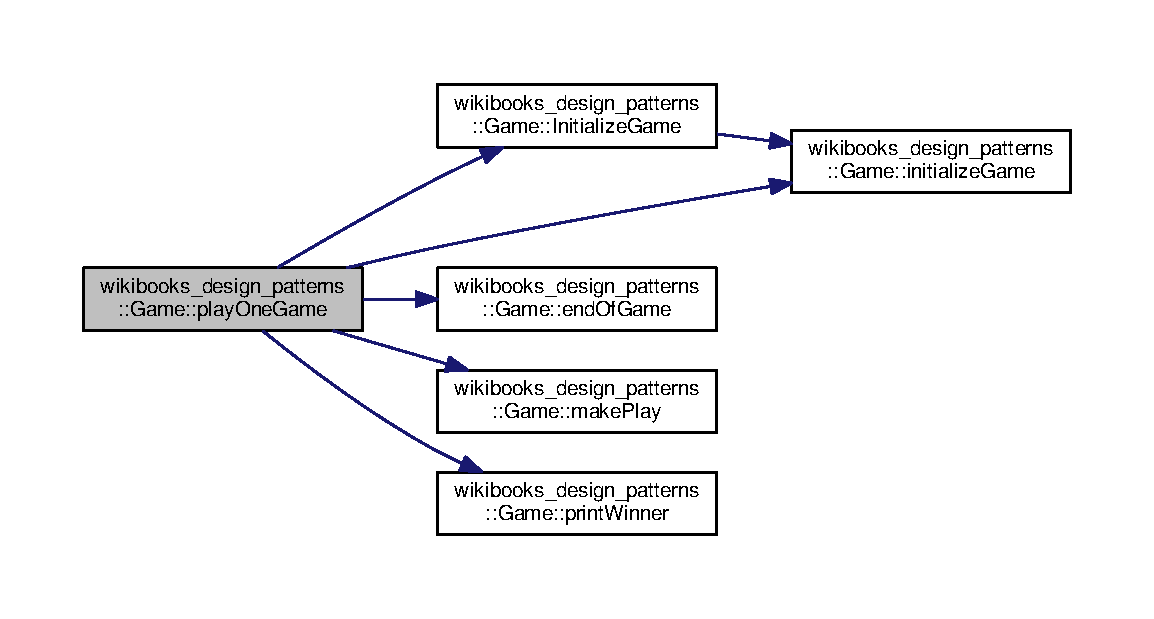
\includegraphics[width=350pt]{classwikibooks__design__patterns_1_1Game_adaf21d3c4d07388f1cba12092ced5d38_cgraph}
\end{center}
\end{figure}


\index{wikibooks\+\_\+design\+\_\+patterns\+::\+Game@{wikibooks\+\_\+design\+\_\+patterns\+::\+Game}!print\+Winner@{print\+Winner}}
\index{print\+Winner@{print\+Winner}!wikibooks\+\_\+design\+\_\+patterns\+::\+Game@{wikibooks\+\_\+design\+\_\+patterns\+::\+Game}}
\subsubsection[{\texorpdfstring{print\+Winner()=0}{printWinner()=0}}]{\setlength{\rightskip}{0pt plus 5cm}virtual void wikibooks\+\_\+design\+\_\+patterns\+::\+Game\+::print\+Winner (
\begin{DoxyParamCaption}
{}
\end{DoxyParamCaption}
)\hspace{0.3cm}{\ttfamily [protected]}, {\ttfamily [pure virtual]}}\hypertarget{classwikibooks__design__patterns_1_1Game_a98d860c143cb793b4c1cb630d9314cba}{}\label{classwikibooks__design__patterns_1_1Game_a98d860c143cb793b4c1cb630d9314cba}


Implemented in \hyperlink{classwikibooks__design__patterns_1_1Chess_a0a38a15831a76736781e8952eeca43d4}{wikibooks\+\_\+design\+\_\+patterns\+::\+Chess}, and \hyperlink{classwikibooks__design__patterns_1_1Monopoly_affb4f25920e5d5887a62b33606bec042}{wikibooks\+\_\+design\+\_\+patterns\+::\+Monopoly}.



\subsection{Member Data Documentation}
\index{wikibooks\+\_\+design\+\_\+patterns\+::\+Game@{wikibooks\+\_\+design\+\_\+patterns\+::\+Game}!moves\+Count@{moves\+Count}}
\index{moves\+Count@{moves\+Count}!wikibooks\+\_\+design\+\_\+patterns\+::\+Game@{wikibooks\+\_\+design\+\_\+patterns\+::\+Game}}
\subsubsection[{\texorpdfstring{moves\+Count}{movesCount}}]{\setlength{\rightskip}{0pt plus 5cm}int wikibooks\+\_\+design\+\_\+patterns\+::\+Game\+::moves\+Count\hspace{0.3cm}{\ttfamily [protected]}}\hypertarget{classwikibooks__design__patterns_1_1Game_ac7bac015fe2e5ead905f7fb8ae63d3aa}{}\label{classwikibooks__design__patterns_1_1Game_ac7bac015fe2e5ead905f7fb8ae63d3aa}
\index{wikibooks\+\_\+design\+\_\+patterns\+::\+Game@{wikibooks\+\_\+design\+\_\+patterns\+::\+Game}!players\+Count@{players\+Count}}
\index{players\+Count@{players\+Count}!wikibooks\+\_\+design\+\_\+patterns\+::\+Game@{wikibooks\+\_\+design\+\_\+patterns\+::\+Game}}
\subsubsection[{\texorpdfstring{players\+Count}{playersCount}}]{\setlength{\rightskip}{0pt plus 5cm}int wikibooks\+\_\+design\+\_\+patterns\+::\+Game\+::players\+Count\hspace{0.3cm}{\ttfamily [protected]}}\hypertarget{classwikibooks__design__patterns_1_1Game_a8641adb02e0f068ff9ecb6c375562d7b}{}\label{classwikibooks__design__patterns_1_1Game_a8641adb02e0f068ff9ecb6c375562d7b}
\index{wikibooks\+\_\+design\+\_\+patterns\+::\+Game@{wikibooks\+\_\+design\+\_\+patterns\+::\+Game}!player\+Won@{player\+Won}}
\index{player\+Won@{player\+Won}!wikibooks\+\_\+design\+\_\+patterns\+::\+Game@{wikibooks\+\_\+design\+\_\+patterns\+::\+Game}}
\subsubsection[{\texorpdfstring{player\+Won}{playerWon}}]{\setlength{\rightskip}{0pt plus 5cm}int wikibooks\+\_\+design\+\_\+patterns\+::\+Game\+::player\+Won\hspace{0.3cm}{\ttfamily [protected]}}\hypertarget{classwikibooks__design__patterns_1_1Game_a6385d85f068769843e22f7741a4ae154}{}\label{classwikibooks__design__patterns_1_1Game_a6385d85f068769843e22f7741a4ae154}


The documentation for this class was generated from the following file\+:\begin{DoxyCompactItemize}
\item 
\hyperlink{Template_8cpp}{Template.\+cpp}\end{DoxyCompactItemize}

\hypertarget{classwikibooks__design__patterns_1_1Monopoly}{}\section{wikibooks\+\_\+design\+\_\+patterns\+:\+:Monopoly Class Reference}
\label{classwikibooks__design__patterns_1_1Monopoly}\index{wikibooks\+\_\+design\+\_\+patterns\+::\+Monopoly@{wikibooks\+\_\+design\+\_\+patterns\+::\+Monopoly}}


Inheritance diagram for wikibooks\+\_\+design\+\_\+patterns\+:\+:Monopoly\+:
\nopagebreak
\begin{figure}[H]
\begin{center}
\leavevmode
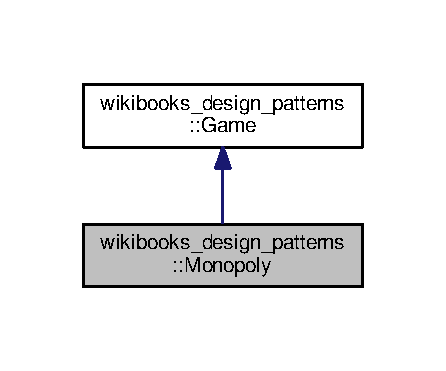
\includegraphics[width=214pt]{classwikibooks__design__patterns_1_1Monopoly__inherit__graph}
\end{center}
\end{figure}


Collaboration diagram for wikibooks\+\_\+design\+\_\+patterns\+:\+:Monopoly\+:
\nopagebreak
\begin{figure}[H]
\begin{center}
\leavevmode
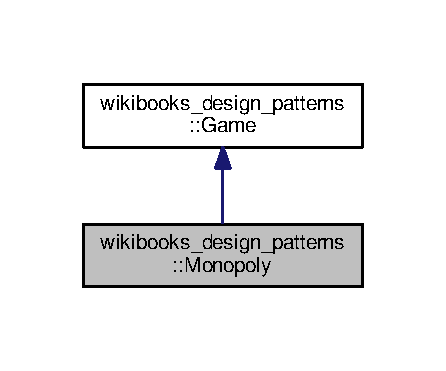
\includegraphics[width=214pt]{classwikibooks__design__patterns_1_1Monopoly__coll__graph}
\end{center}
\end{figure}
\subsection*{Private Types}
\begin{DoxyCompactItemize}
\item 
enum \{ \hyperlink{classwikibooks__design__patterns_1_1Monopoly_a503a2b1818164ca11be7cc029dcc84e6a7f717a5237abe25eac65acce1a12d2f3}{M\+O\+V\+E\+S\+\_\+\+W\+I\+N\+\_\+\+C\+O\+R\+R\+E\+C\+T\+I\+ON} = 20
 \}
\end{DoxyCompactItemize}
\subsection*{Private Member Functions}
\begin{DoxyCompactItemize}
\item 
void \hyperlink{classwikibooks__design__patterns_1_1Monopoly_a9fa4e1a5c85d7b9f1e2b1fdf4d1911ab}{initialize\+Game} ()
\item 
void \hyperlink{classwikibooks__design__patterns_1_1Monopoly_ab885dd62ab49fba54bd2ce542702caaa}{make\+Play} (int player)
\item 
bool \hyperlink{classwikibooks__design__patterns_1_1Monopoly_ab533fb92f64065d8cae9a731e6fe789d}{end\+Of\+Game} ()
\item 
void \hyperlink{classwikibooks__design__patterns_1_1Monopoly_affb4f25920e5d5887a62b33606bec042}{print\+Winner} ()
\end{DoxyCompactItemize}
\subsection*{Additional Inherited Members}


\subsection{Member Enumeration Documentation}
\subsubsection[{\texorpdfstring{anonymous enum}{anonymous enum}}]{\setlength{\rightskip}{0pt plus 5cm}anonymous enum\hspace{0.3cm}{\ttfamily [private]}}\hypertarget{classwikibooks__design__patterns_1_1Monopoly_a503a2b1818164ca11be7cc029dcc84e6}{}\label{classwikibooks__design__patterns_1_1Monopoly_a503a2b1818164ca11be7cc029dcc84e6}
\begin{Desc}
\item[Enumerator]\par
\begin{description}
\index{M\+O\+V\+E\+S\+\_\+\+W\+I\+N\+\_\+\+C\+O\+R\+R\+E\+C\+T\+I\+ON@{M\+O\+V\+E\+S\+\_\+\+W\+I\+N\+\_\+\+C\+O\+R\+R\+E\+C\+T\+I\+ON}!wikibooks\+\_\+design\+\_\+patterns\+::\+Monopoly@{wikibooks\+\_\+design\+\_\+patterns\+::\+Monopoly}}\index{wikibooks\+\_\+design\+\_\+patterns\+::\+Monopoly@{wikibooks\+\_\+design\+\_\+patterns\+::\+Monopoly}!M\+O\+V\+E\+S\+\_\+\+W\+I\+N\+\_\+\+C\+O\+R\+R\+E\+C\+T\+I\+ON@{M\+O\+V\+E\+S\+\_\+\+W\+I\+N\+\_\+\+C\+O\+R\+R\+E\+C\+T\+I\+ON}}\item[{\em 
M\+O\+V\+E\+S\+\_\+\+W\+I\+N\+\_\+\+C\+O\+R\+R\+E\+C\+T\+I\+ON\hypertarget{classwikibooks__design__patterns_1_1Monopoly_a503a2b1818164ca11be7cc029dcc84e6a7f717a5237abe25eac65acce1a12d2f3}{}\label{classwikibooks__design__patterns_1_1Monopoly_a503a2b1818164ca11be7cc029dcc84e6a7f717a5237abe25eac65acce1a12d2f3}
}]\end{description}
\end{Desc}

\begin{DoxyCode}
103     \{
104         \hyperlink{classwikibooks__design__patterns_1_1Monopoly_a503a2b1818164ca11be7cc029dcc84e6a7f717a5237abe25eac65acce1a12d2f3}{MOVES\_WIN\_CORRECTION} = 20,
105     \};
\end{DoxyCode}


\subsection{Member Function Documentation}
\index{wikibooks\+\_\+design\+\_\+patterns\+::\+Monopoly@{wikibooks\+\_\+design\+\_\+patterns\+::\+Monopoly}!end\+Of\+Game@{end\+Of\+Game}}
\index{end\+Of\+Game@{end\+Of\+Game}!wikibooks\+\_\+design\+\_\+patterns\+::\+Monopoly@{wikibooks\+\_\+design\+\_\+patterns\+::\+Monopoly}}
\subsubsection[{\texorpdfstring{end\+Of\+Game()}{endOfGame()}}]{\setlength{\rightskip}{0pt plus 5cm}bool wikibooks\+\_\+design\+\_\+patterns\+::\+Monopoly\+::end\+Of\+Game (
\begin{DoxyParamCaption}
{}
\end{DoxyParamCaption}
)\hspace{0.3cm}{\ttfamily [inline]}, {\ttfamily [private]}, {\ttfamily [virtual]}}\hypertarget{classwikibooks__design__patterns_1_1Monopoly_ab533fb92f64065d8cae9a731e6fe789d}{}\label{classwikibooks__design__patterns_1_1Monopoly_ab533fb92f64065d8cae9a731e6fe789d}


Implements \hyperlink{classwikibooks__design__patterns_1_1Game_a351f5fb200c6b26d5b6150f1f09bc87d}{wikibooks\+\_\+design\+\_\+patterns\+::\+Game}.


\begin{DoxyCode}
88                      \{
89         \textcolor{comment}{// Return true if game is over }
90         \textcolor{comment}{// according to Monopoly rules}
91     \textcolor{keywordflow}{return} (-1 != \hyperlink{classwikibooks__design__patterns_1_1Game_a6385d85f068769843e22f7741a4ae154}{playerWon});
92     \}
\end{DoxyCode}
\index{wikibooks\+\_\+design\+\_\+patterns\+::\+Monopoly@{wikibooks\+\_\+design\+\_\+patterns\+::\+Monopoly}!initialize\+Game@{initialize\+Game}}
\index{initialize\+Game@{initialize\+Game}!wikibooks\+\_\+design\+\_\+patterns\+::\+Monopoly@{wikibooks\+\_\+design\+\_\+patterns\+::\+Monopoly}}
\subsubsection[{\texorpdfstring{initialize\+Game()}{initializeGame()}}]{\setlength{\rightskip}{0pt plus 5cm}void wikibooks\+\_\+design\+\_\+patterns\+::\+Monopoly\+::initialize\+Game (
\begin{DoxyParamCaption}
{}
\end{DoxyParamCaption}
)\hspace{0.3cm}{\ttfamily [inline]}, {\ttfamily [private]}, {\ttfamily [virtual]}}\hypertarget{classwikibooks__design__patterns_1_1Monopoly_a9fa4e1a5c85d7b9f1e2b1fdf4d1911ab}{}\label{classwikibooks__design__patterns_1_1Monopoly_a9fa4e1a5c85d7b9f1e2b1fdf4d1911ab}


Implements \hyperlink{classwikibooks__design__patterns_1_1Game_a77c50ee852af77bb15d46ba0a39683c4}{wikibooks\+\_\+design\+\_\+patterns\+::\+Game}.


\begin{DoxyCode}
72                           \{
73         \textcolor{comment}{// Initialize players}
74     \hyperlink{classwikibooks__design__patterns_1_1Game_a8641adb02e0f068ff9ecb6c375562d7b}{playersCount} = rand() * 7 / RAND\_MAX + 2;
75         \textcolor{comment}{// Initialize money}
76     \}
\end{DoxyCode}
\index{wikibooks\+\_\+design\+\_\+patterns\+::\+Monopoly@{wikibooks\+\_\+design\+\_\+patterns\+::\+Monopoly}!make\+Play@{make\+Play}}
\index{make\+Play@{make\+Play}!wikibooks\+\_\+design\+\_\+patterns\+::\+Monopoly@{wikibooks\+\_\+design\+\_\+patterns\+::\+Monopoly}}
\subsubsection[{\texorpdfstring{make\+Play(int player)}{makePlay(int player)}}]{\setlength{\rightskip}{0pt plus 5cm}void wikibooks\+\_\+design\+\_\+patterns\+::\+Monopoly\+::make\+Play (
\begin{DoxyParamCaption}
\item[{int}]{player}
\end{DoxyParamCaption}
)\hspace{0.3cm}{\ttfamily [inline]}, {\ttfamily [private]}, {\ttfamily [virtual]}}\hypertarget{classwikibooks__design__patterns_1_1Monopoly_ab885dd62ab49fba54bd2ce542702caaa}{}\label{classwikibooks__design__patterns_1_1Monopoly_ab885dd62ab49fba54bd2ce542702caaa}


Implements \hyperlink{classwikibooks__design__patterns_1_1Game_ab1859f681536780d02da57634e963d4a}{wikibooks\+\_\+design\+\_\+patterns\+::\+Game}.


\begin{DoxyCode}
77                               \{
78         \textcolor{comment}{// Process one turn of player}
79 
80     \textcolor{comment}{//  Decide winner}
81     \textcolor{keywordflow}{if} (\hyperlink{classwikibooks__design__patterns_1_1Game_ac7bac015fe2e5ead905f7fb8ae63d3aa}{movesCount} < 20)
82         \textcolor{keywordflow}{return};
83     \textcolor{keyword}{const} \textcolor{keywordtype}{int} chances = (\hyperlink{classwikibooks__design__patterns_1_1Game_ac7bac015fe2e5ead905f7fb8ae63d3aa}{movesCount} > 199) ? 199 : \hyperlink{classwikibooks__design__patterns_1_1Game_ac7bac015fe2e5ead905f7fb8ae63d3aa}{movesCount};
84     \textcolor{keyword}{const} \textcolor{keywordtype}{int} random = \hyperlink{classwikibooks__design__patterns_1_1Monopoly_a503a2b1818164ca11be7cc029dcc84e6a7f717a5237abe25eac65acce1a12d2f3}{MOVES\_WIN\_CORRECTION} * rand() * 200 / RAND\_MAX;
85     \textcolor{keywordflow}{if} (random < chances)
86         \hyperlink{classwikibooks__design__patterns_1_1Game_a6385d85f068769843e22f7741a4ae154}{playerWon} = player;
87     \}
\end{DoxyCode}
\index{wikibooks\+\_\+design\+\_\+patterns\+::\+Monopoly@{wikibooks\+\_\+design\+\_\+patterns\+::\+Monopoly}!print\+Winner@{print\+Winner}}
\index{print\+Winner@{print\+Winner}!wikibooks\+\_\+design\+\_\+patterns\+::\+Monopoly@{wikibooks\+\_\+design\+\_\+patterns\+::\+Monopoly}}
\subsubsection[{\texorpdfstring{print\+Winner()}{printWinner()}}]{\setlength{\rightskip}{0pt plus 5cm}void wikibooks\+\_\+design\+\_\+patterns\+::\+Monopoly\+::print\+Winner (
\begin{DoxyParamCaption}
{}
\end{DoxyParamCaption}
)\hspace{0.3cm}{\ttfamily [inline]}, {\ttfamily [private]}, {\ttfamily [virtual]}}\hypertarget{classwikibooks__design__patterns_1_1Monopoly_affb4f25920e5d5887a62b33606bec042}{}\label{classwikibooks__design__patterns_1_1Monopoly_affb4f25920e5d5887a62b33606bec042}


Implements \hyperlink{classwikibooks__design__patterns_1_1Game_a98d860c143cb793b4c1cb630d9314cba}{wikibooks\+\_\+design\+\_\+patterns\+::\+Game}.


\begin{DoxyCode}
93                        \{
94     assert(\hyperlink{classwikibooks__design__patterns_1_1Game_a6385d85f068769843e22f7741a4ae154}{playerWon} >= 0);
95     assert(\hyperlink{classwikibooks__design__patterns_1_1Game_a6385d85f068769843e22f7741a4ae154}{playerWon} < \hyperlink{classwikibooks__design__patterns_1_1Game_a8641adb02e0f068ff9ecb6c375562d7b}{playersCount});
96 
97         \textcolor{comment}{// Display who won}
98     std::cout<<\textcolor{stringliteral}{"Monopoly, player "}<<\hyperlink{classwikibooks__design__patterns_1_1Game_a6385d85f068769843e22f7741a4ae154}{playerWon}<<\textcolor{stringliteral}{" won in "}<<\hyperlink{classwikibooks__design__patterns_1_1Game_ac7bac015fe2e5ead905f7fb8ae63d3aa}{movesCount}<<\textcolor{stringliteral}{" moves."}<<
      std::endl;
99     \}
\end{DoxyCode}


The documentation for this class was generated from the following file\+:\begin{DoxyCompactItemize}
\item 
\hyperlink{Template_8cpp}{Template.\+cpp}\end{DoxyCompactItemize}

\chapter{File Documentation}
\hypertarget{Template_8cpp}{}\section{Template.\+cpp File Reference}
\label{Template_8cpp}\index{Template.\+cpp@{Template.\+cpp}}
{\ttfamily \#include $<$ctime$>$}\\*
{\ttfamily \#include $<$assert.\+h$>$}\\*
{\ttfamily \#include $<$iostream$>$}\\*
Include dependency graph for Template.\+cpp\+:
\nopagebreak
\begin{figure}[H]
\begin{center}
\leavevmode
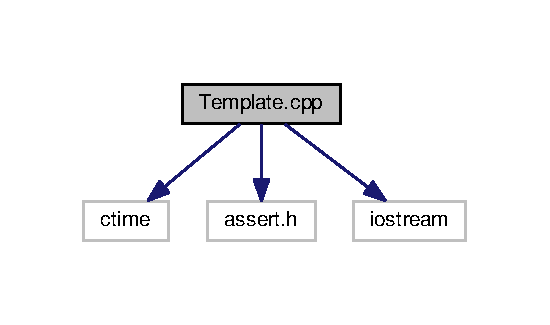
\includegraphics[width=264pt]{Template_8cpp__incl}
\end{center}
\end{figure}
\subsection*{Classes}
\begin{DoxyCompactItemize}
\item 
class \hyperlink{classwikibooks__design__patterns_1_1Game}{wikibooks\+\_\+design\+\_\+patterns\+::\+Game}
\item 
class \hyperlink{classwikibooks__design__patterns_1_1Monopoly}{wikibooks\+\_\+design\+\_\+patterns\+::\+Monopoly}
\item 
class \hyperlink{classwikibooks__design__patterns_1_1Chess}{wikibooks\+\_\+design\+\_\+patterns\+::\+Chess}
\end{DoxyCompactItemize}
\subsection*{Namespaces}
\begin{DoxyCompactItemize}
\item 
 \hyperlink{namespacewikibooks__design__patterns}{wikibooks\+\_\+design\+\_\+patterns}
\end{DoxyCompactItemize}
\subsection*{Functions}
\begin{DoxyCompactItemize}
\item 
int \hyperlink{Template_8cpp_ae66f6b31b5ad750f1fe042a706a4e3d4}{main} ()
\end{DoxyCompactItemize}


\subsection{Function Documentation}
\index{Template.\+cpp@{Template.\+cpp}!main@{main}}
\index{main@{main}!Template.\+cpp@{Template.\+cpp}}
\subsubsection[{\texorpdfstring{main()}{main()}}]{\setlength{\rightskip}{0pt plus 5cm}int main (
\begin{DoxyParamCaption}
{}
\end{DoxyParamCaption}
)}\hypertarget{Template_8cpp_ae66f6b31b5ad750f1fe042a706a4e3d4}{}\label{Template_8cpp_ae66f6b31b5ad750f1fe042a706a4e3d4}

\begin{DoxyCode}
153 \{
154     \textcolor{keyword}{using namespace }\hyperlink{namespacewikibooks__design__patterns}{wikibooks\_design\_patterns};
155 
156     \hyperlink{classwikibooks__design__patterns_1_1Game}{Game}* game = NULL;
157 
158     \hyperlink{classwikibooks__design__patterns_1_1Chess}{Chess} chess;
159     game = &chess;
160     \textcolor{keywordflow}{for} (\textcolor{keywordtype}{unsigned} i = 0; i < 100; ++i)
161      game->\hyperlink{classwikibooks__design__patterns_1_1Game_adaf21d3c4d07388f1cba12092ced5d38}{playOneGame}();
162 
163     \hyperlink{classwikibooks__design__patterns_1_1Monopoly}{Monopoly} monopoly;
164     game = &monopoly;
165     \textcolor{keywordflow}{for} (\textcolor{keywordtype}{unsigned} i = 0; i < 100; ++i)
166     game->\hyperlink{classwikibooks__design__patterns_1_1Game_adaf21d3c4d07388f1cba12092ced5d38}{playOneGame}();
167 
168     \textcolor{keywordflow}{return} 0;
169 \}\end{DoxyCode}


Here is the call graph for this function\+:
\nopagebreak
\begin{figure}[H]
\begin{center}
\leavevmode
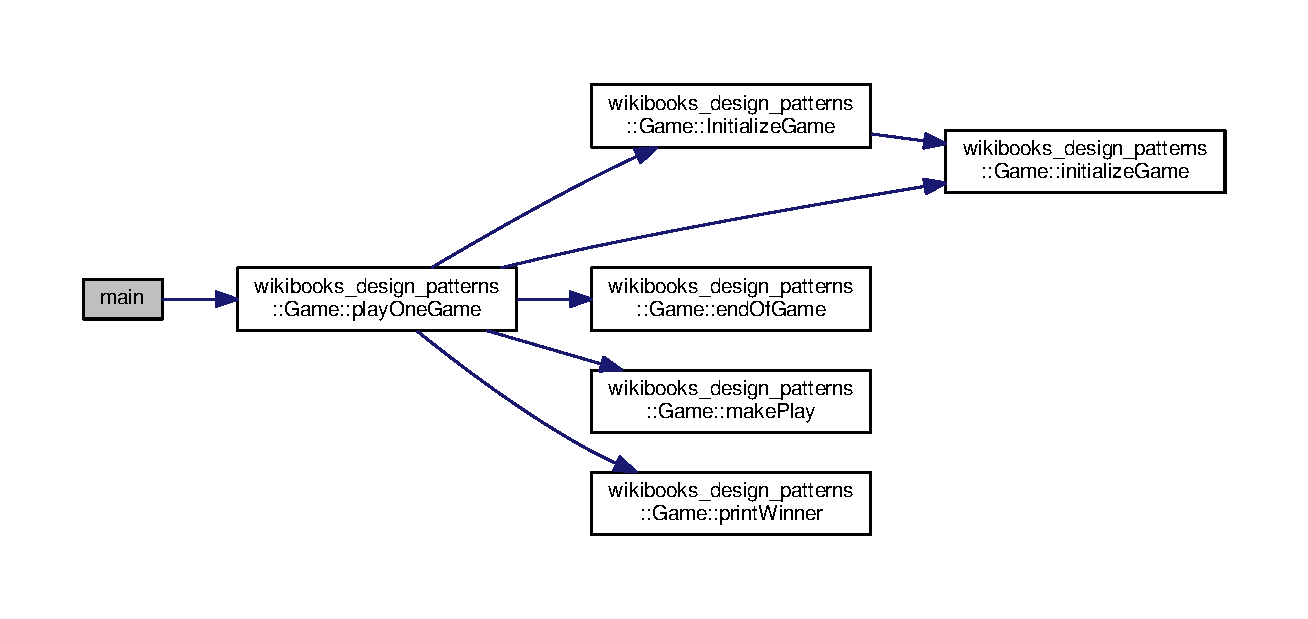
\includegraphics[width=350pt]{Template_8cpp_ae66f6b31b5ad750f1fe042a706a4e3d4_cgraph}
\end{center}
\end{figure}



%--- End generated contents ---

% Index
\backmatter
\newpage
\phantomsection
\clearemptydoublepage
\addcontentsline{toc}{chapter}{Index}
\printindex

\end{document}
